\documentclass[12pt,a4paper]{article}
\usepackage[utf8]{inputenc}
\usepackage[spanish,es-tabla]{babel}
\usepackage{geometry}
\usepackage{graphicx}
\usepackage{multirow}
\usepackage{tabularx}
\usepackage{mathptmx}
\usepackage{fancyhdr}
\usepackage{array}
\usepackage[table]{xcolor}
\usepackage{titlesec}
\usepackage{setspace}
\usepackage{microtype}
\usepackage{lastpage}
\usepackage{booktabs}
\usepackage{enumitem}
\usepackage{amsmath}
\usepackage{amsfonts}
\usepackage{amssymb}

\usepackage{float}
\usepackage{placeins}
\usepackage{tikz}
\usepackage{pgfplots}
\pgfplotsset{compat=1.17}
\usetikzlibrary{arrows.meta,positioning,shapes.geometric,calc}

\graphicspath{{images/}{../images/}{./}}

\geometry{
    top=4.7cm,
    bottom=2.5cm,
    left=2.5cm,
    right=2.5cm,
    headheight=3.9cm,
    headsep=0.4cm
}

\setstretch{1.15}
\setlength{\parindent}{0pt}
\setlength{\parskip}{0.45em}
\setlength{\tabcolsep}{4pt}

\titleformat{\section}
  {\normalfont\fontsize{12}{14.5}\bfseries}{\thesection.}{0.6em}{\uppercase}
\titlespacing*{\section}
  {0pt}{1.8ex plus 0.4ex minus 0.2ex}{0.6ex plus 0.2ex}

\titleformat{\subsection}
  {\normalfont\fontsize{11.5}{13.5}\bfseries}{\thesubsection.}{0.5em}{}
\titlespacing*{\subsection}
  {0pt}{1.4ex plus 0.3ex minus 0.1ex}{0.4ex plus 0.1ex}

\titleformat{\subsubsection}
  {\normalfont\fontsize{10.5}{12.5}\bfseries\itshape}{\thesubsubsection.}{0.4em}{}
\titlespacing*{\subsubsection}
  {0pt}{1.1ex plus 0.2ex minus 0.1ex}{0.3ex plus 0.1ex}

\newcolumntype{Y}{>{\centering\arraybackslash}X}
\newcolumntype{L}{>{\raggedright\arraybackslash}X}
\newcolumntype{C}{>{\centering\arraybackslash}X}

\definecolor{headerblue}{RGB}{26, 54, 93}
\definecolor{darkblue}{RGB}{43, 108, 176}
\definecolor{lightgraybg}{RGB}{248, 248, 248}
\definecolor{tableheader}{RGB}{232, 238, 246}
\definecolor{navyheader}{RGB}{0, 32, 96}
\definecolor{lineblue}{RGB}{0, 102, 204}
\definecolor{areablue}{RGB}{220, 236, 252}
\definecolor{lcsred}{RGB}{217, 56, 41}
\definecolor{lcigreen}{RGB}{46, 125, 50}
\definecolor{lciorange}{RGB}{230, 81, 0}
\definecolor{ishikawared}{RGB}{160, 0, 0}

\tikzset{
    catbox/.style={draw, fill=tableheader, font=\footnotesize\bfseries, minimum width=2.8cm, minimum height=0.65cm, align=center},
    efectobox/.style={draw=ishikawared!90!black, line width=1.2pt, fill=ishikawared, text=white, font=\small\bfseries, align=center, inner sep=6pt, text width=3.8cm},
    causetext/.style={font=\scriptsize, align=right, text=black!90}
}

\newcommand{\docCodigo}{TI-SIGE-ENT-F3-003}
\newcommand{\docVersion}{1.0}
\newcommand{\docProceso}{IMPLEMENTACIÓN DE SOFTWARE / SEGURIDAD Y CONTROL DE ACCESO}
\newcommand{\docElaboracion}{11/09/2026}
\newcommand{\docRevision}{11/09/2026}
\newcommand{\docTitulo}{AUTENTICACIÓN Y AUTORIZACIÓN DE USUARIOS}
\newcommand{\docOrganizacion}{FACULTAD DE INGENIERÍA EN SISTEMAS, ELECTRÓNICA E INDUSTRIAL}
\newcommand{\docSubOrganizacion}{CARRERA DE INGENIERÍA DE SOFTWARE}

\newcommand{\encabezadofrecuente}{%
    \renewcommand{\arraystretch}{1.15}%
    \noindent\makebox[\textwidth][c]{%
    \begin{tabularx}{\textwidth}{|>{\centering\arraybackslash}m{2.8cm}|Y|>{\centering\arraybackslash}m{4.8cm}|}
        \hline
        \multirow{4}{2.8cm}{\centering\raisebox{-1.15cm}{
\includegraphics[width=2.5cm,height=2.0cm,keepaspectratio]{images/logo.png}}}
        & \textbf{\fontsize{9}{11}\selectfont \docOrganizacion} 
        & \textbf{\fontsize{8}{10}\selectfont CÓDIGO:} \fontsize{8}{10}\selectfont \docCodigo \\
        \cline{3-3}
        & \textbf{\fontsize{8.5}{10.5}\selectfont \docSubOrganizacion} 
        & \textbf{\fontsize{8}{10}\selectfont VERSIÓN:} \fontsize{8}{10}\selectfont \docVersion \\
        \cline{2-3}
        & \textbf{\fontsize{8}{10}\selectfont PROCESO:} \fontsize{8}{10}\selectfont \docProceso 
        & \textbf{\fontsize{8}{10}\selectfont ELABORACIÓN:} \fontsize{8}{10}\selectfont \docElaboracion \\
        \cline{2-3}
        & \textbf{\fontsize{8.5}{10.5}\selectfont \docTitulo} 
        & \textbf{\fontsize{8}{10}\selectfont ÚLTIMA REVISIÓN:} \fontsize{8}{10}\selectfont \docRevision \\
        \hline
    \end{tabularx}%
    }%
}

\pagestyle{fancy}
\fancyhf{}
\fancyhead[C]{\encabezadofrecuente}
\fancyfoot[C]{\fontsize{10}{12}\selectfont Página \thepage\ de \pageref{LastPage}}
\renewcommand{\headrulewidth}{0pt}

\begin{document}

\noindent{\fontsize{10.5}{12.5}\selectfont \textbf{Integrantes:} Heidi Villavicencio \quad$\vert$\quad Steeven Toala \quad$\vert$\quad Nixon Hurtado \quad$\vert$\quad Andrea Vásquez}

\vspace{0.25cm}

\section{Título}
\textbf{Denominación Oficial del Entregable:} Autenticación y Autorización de Usuarios -- Código EDT: 3.3

\section{Introducción}
La seguridad en el acceso a la plataforma SIGE es un requerimiento crítico dado que gestiona planes de trabajo institucionales, evaluaciones y firmas digitales vinculantes. Este entregable documenta la implementación completa del subsistema de autenticación y autorización basado en tokens web JSON (JWT) y control de acceso basado en roles (RBAC). Se detallan los mecanismos de generación de tokens firmados mediante algoritmo HMAC-SHA256, el flujo de refresco de credenciales, el almacenamiento seguro de contraseñas con Argon2id y la protección de rutas tanto a nivel de middleware en Express v5 como en el enrutador cliente en React.

\section{Objetivo}
\subsection{Objetivo General}
Implementar el subsistema de autenticación y autorización segura con JWT y RBAC en el backend y frontend de SIGE, garantizando la delimitación estricta de privilegios.
\subsection{Objetivos Específicos}
\begin{itemize}[leftmargin=1.5em, itemsep=2pt]
    \item Desarrollar los endpoints de login (\texttt{POST /api/auth/login}) y verificación (\texttt{GET /api/auth/me}).
    \item Construir los middlewares de Express para validación de token y autorización por roles.
    \item Diseñar e integrar la vista interactiva de inicio de sesión en el cliente React.
\end{itemize}

\section{Alcance}
\subsection{Límites del Entregable (In-Scope)}
\begin{itemize}[leftmargin=1.5em, itemsep=2pt]
    \item Protección de todos los endpoints de la API REST mediante autorización por encabezado \texttt{Authorization: Bearer <token>}.
    \item Integración visual y manejo de estado de sesión en el frontend con \texttt{AuthContext.jsx}.
\end{itemize}
\subsection{Exclusiones (Out-of-Scope)}
\begin{itemize}[leftmargin=1.5em, itemsep=2pt]
    \item Integración con directorio activo LDAP institucional universitario (previsto como módulo de sincronización futura).
\end{itemize}

\section{Definiciones}
\begin{itemize}[leftmargin=1.5em, itemsep=2pt]
    \item \textbf{JWT (JSON Web Token):} Estándar RFC 7519 para transmitir de forma segura información compacta y autónoma entre partes como objeto JSON.
    \item \textbf{RBAC (Role-Based Access Control):} Mecanismo de restricción de accesos a recursos del sistema en función de los roles asignados a los usuarios.
    \item \textbf{Argon2id:} Algoritmo moderno ganador de la Password Hashing Competition altamente resistente a ataques GPU y side-channel.
\end{itemize}

\section{Responsabilidades}
\begin{itemize}[leftmargin=1.5em, itemsep=2pt]
    \item \textbf{Steeven Toala (Responsable EDT 3.3):} Implementación de endpoints de autenticación, JWT y middleware RBAC.
    \item \textbf{Heidi Villavicencio (Diseñadora UI):} Diseño e implementación visual del formulario de login accesible.
    \item \textbf{Ing. Paulo Torres (Docente Evaluador):} Auditoría de seguridad del mecanismo de autenticación.
\end{itemize}

\section{Normativa Legal y Técnica}
\subsection{Marco Legal Ecuatoriano}
\begin{itemize}[leftmargin=1.5em, itemsep=2pt]
    \item \textbf{Ley Orgánica de Protección de Datos Personales (LOPDP), Art. 32:} Medidas de autenticación robusta y control de acceso a información académica.
    \item \textbf{Esquema Gubernamental de Seguridad de la Información (EGSI):} Políticas de complejidad y almacenamiento irreversible de contraseñas.
\end{itemize}
\subsection{Normas Técnicas Internacionales}
\begin{itemize}[leftmargin=1.5em, itemsep=2pt]
    \item \textbf{RFC 7519 (JSON Web Token):} Especificación técnica de estructura y firma de tokens de acceso.
    \item \textbf{OWASP ASVS v4.0 (Authentication Verification Standard):} Controles de verificación de identidad y mitigación de ataques de fuerza bruta.
\end{itemize}

\section{Método, Políticas y Contenidos}
\subsection{Enfoque Metodológico}
Se implementó un esquema de autenticación sin estado (\textit{stateless}). Al autenticarse, el usuario recibe un Access Token con tiempo de expiración corto (15 minutos) que contiene su identificador, correo y lista de roles. Para mitigar ataques de fuerza bruta, se integró el middleware \texttt{express-rate-limit} restringiendo a 5 intentos fallidos por dirección IP en una ventana de 15 minutos. En el cliente, el token se custodia en memoria mediante React Context, con respaldo en \texttt{sessionStorage} para persistir recargas de pestaña.

\subsection{Políticas de Calidad de Seguridad}
\begin{enumerate}[leftmargin=1.5em, itemsep=2pt]
    \item \textbf{Política de Expiración Estricta de Tokens:} Los access tokens expiran en exactamente 15 minutos, forzando la revalidación continua de privilegios.
    \item \textbf{Política de Bloqueo por Fuerza Bruta:} Tras 5 intentos consecutivos erróneos, la cuenta queda bloqueada temporalmente durante 15 minutos.
    \item \textbf{Política de Cifrado Irreversible:} Las contraseñas se almacenan procesadas exclusivamente con Argon2id con salt aleatorio de 16 bytes.
    \item \textbf{Política de Principio de Menor Privilegio:} Ninguna ruta protegida permite acceso sin comprobar explícitamente el rol mínimo requerido en el decorador o middleware.
\end{enumerate}

\begin{figure}[H]
    \centering
    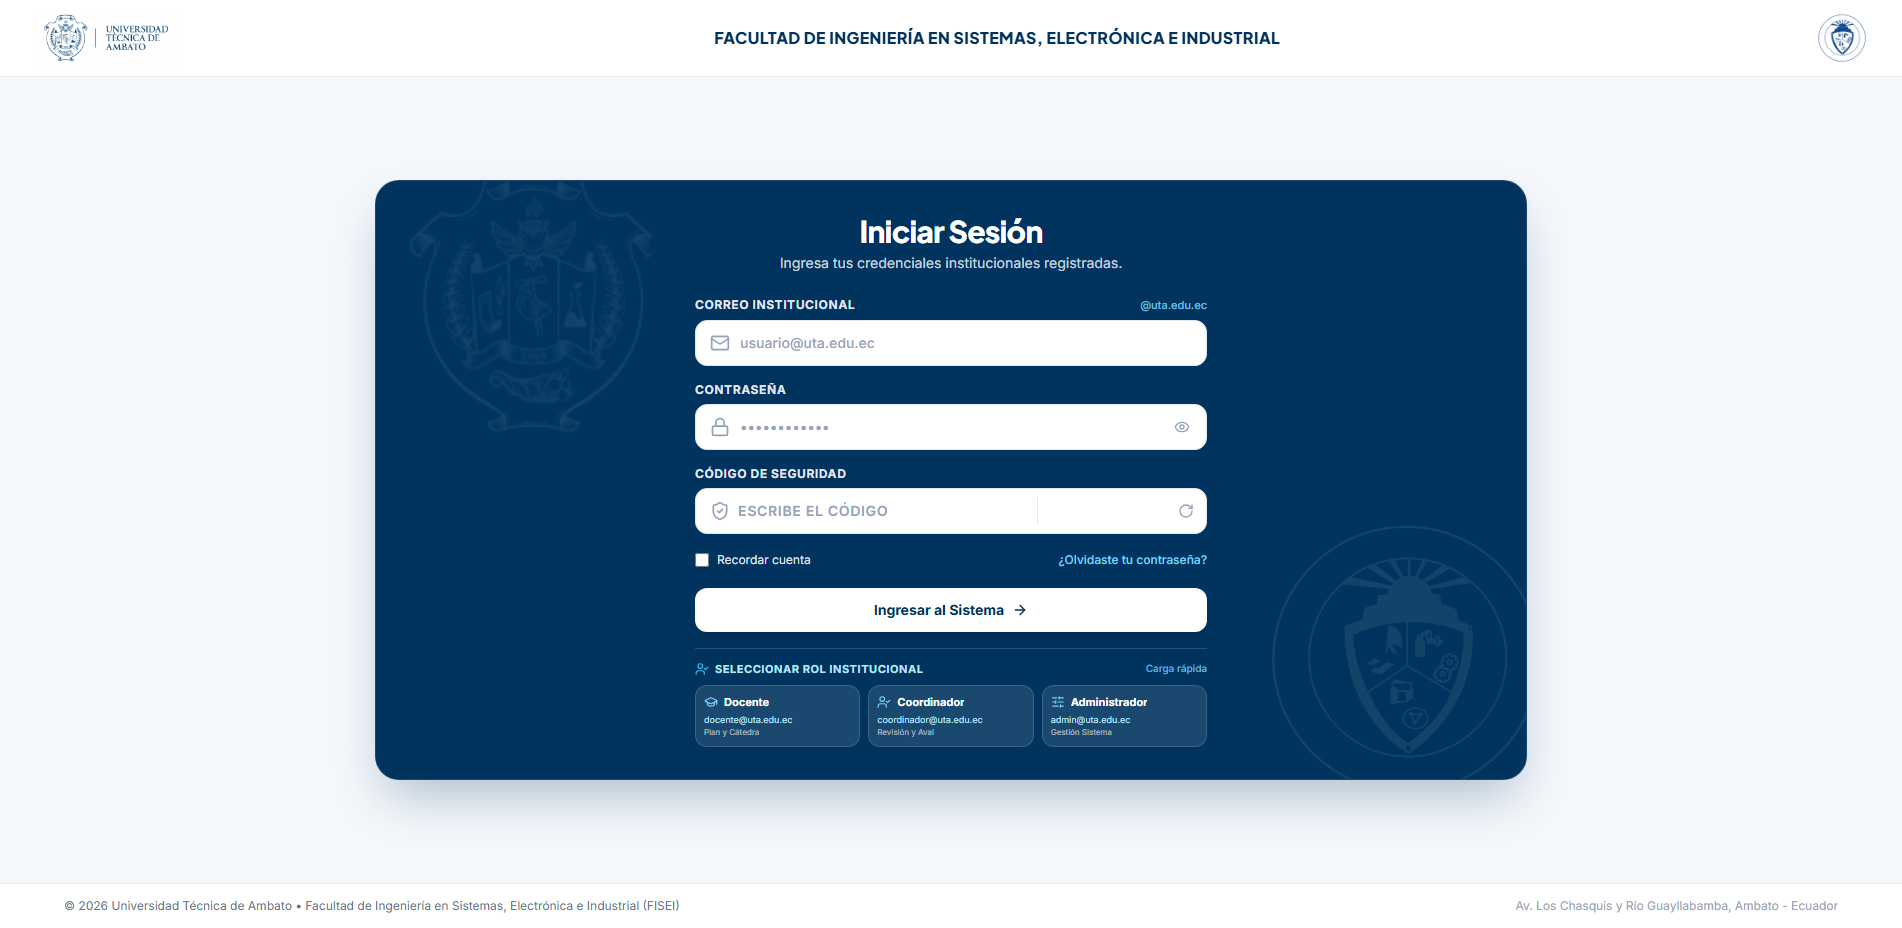
\includegraphics[width=0.88\textwidth,height=5.8cm,keepaspectratio]{images/sige_login_view.png}
    \caption{Captura Real de la Pantalla de Inicio de Sesión y Autenticación del Sistema SIGE.}
    \label{fig:login_screen}
\end{figure}
\FloatBarrier

\begin{figure}[H]
    \centering
    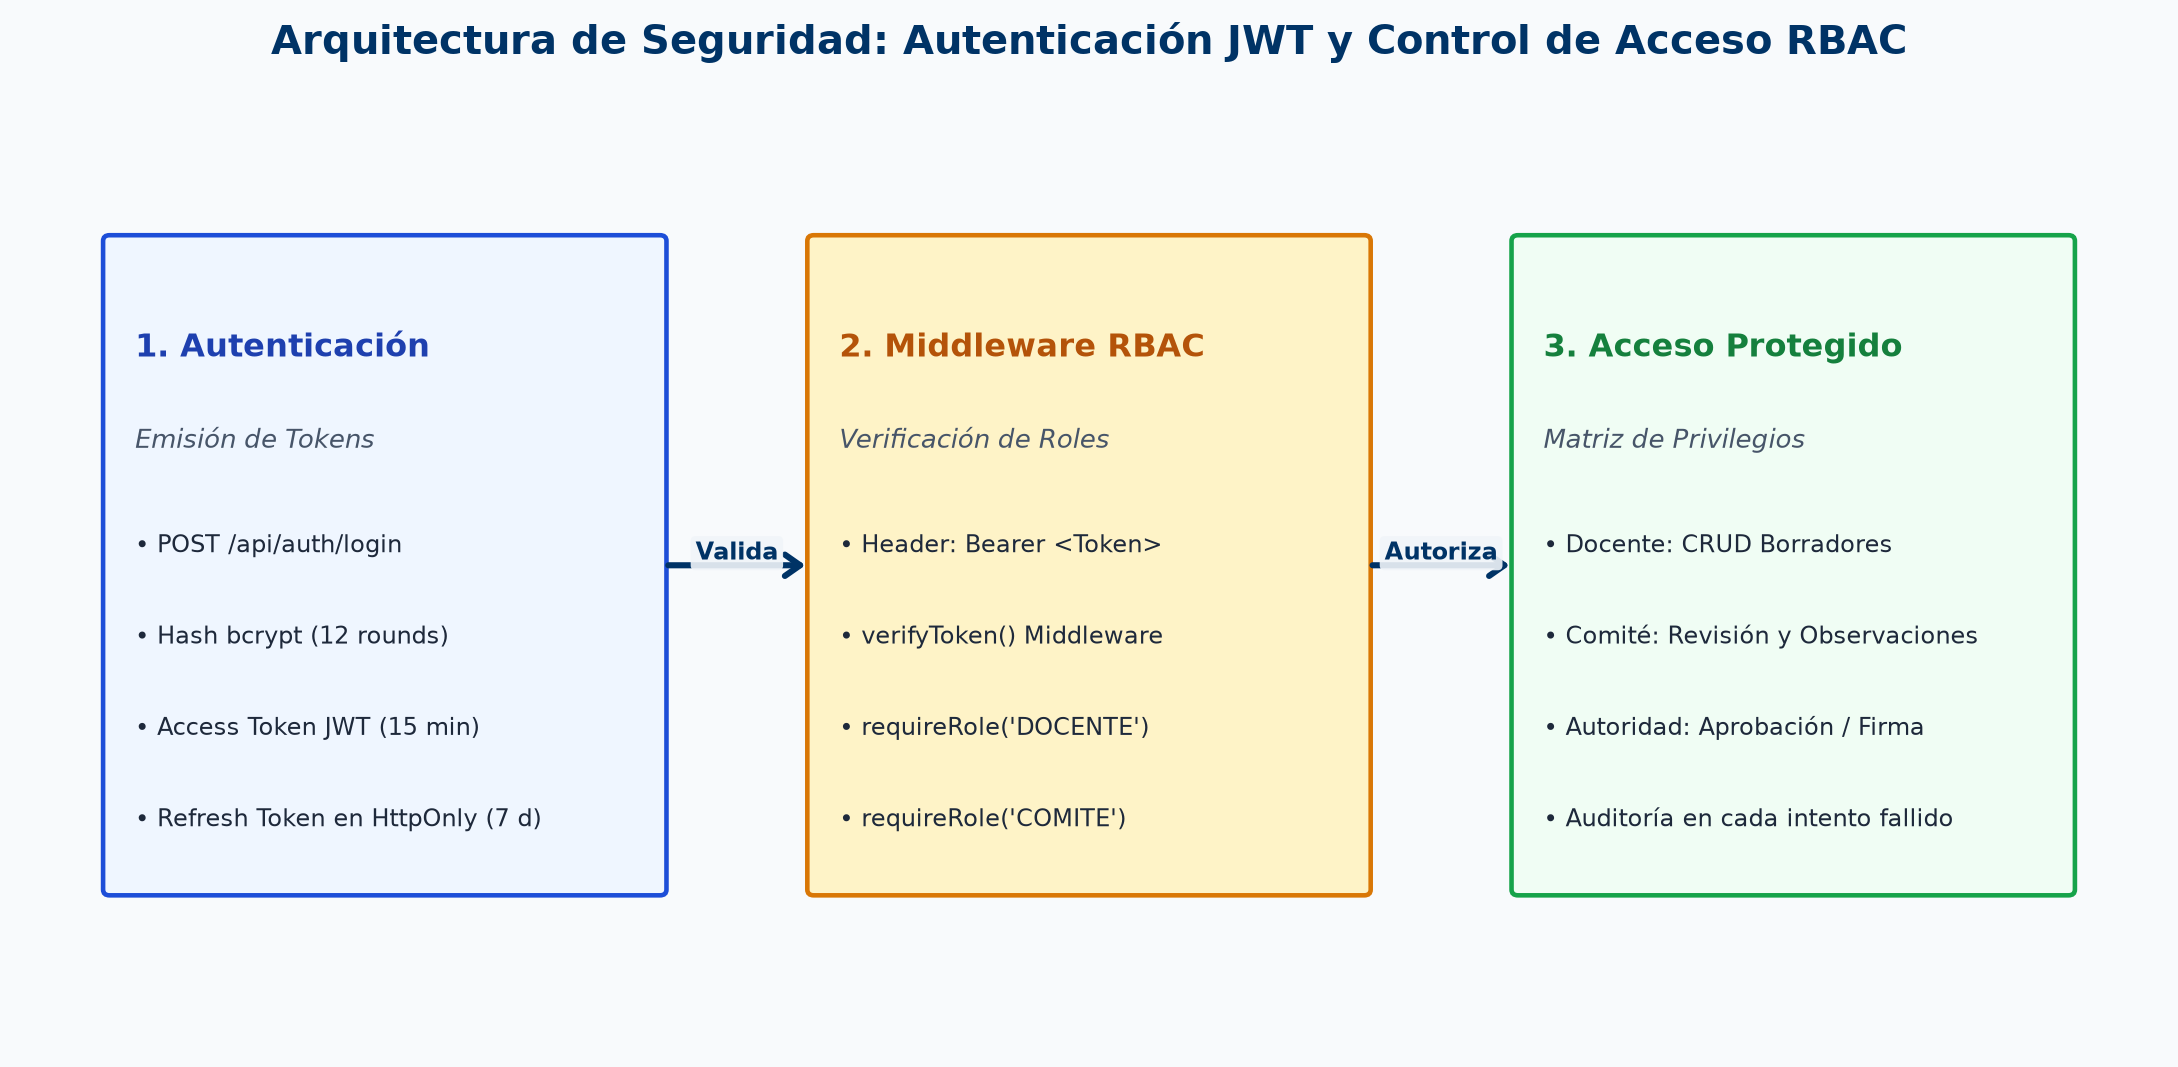
\includegraphics[width=0.88\textwidth,height=5.6cm,keepaspectratio]{images/f3_03_seguridad_jwt_rbac.png}
    \caption{Arquitectura de Intercambio de Tokens JWT y Middleware RBAC en Backend Express v5.}
    \label{fig:jwt_rbac}
\end{figure}
\FloatBarrier

\section{Descripción de actividades}
\subsection{Matriz de Control de Acceso por Roles (RBAC Matrix)}
\begin{table}[H]
\centering
\small
\renewcommand{\arraystretch}{1.2}
\begin{tabularx}{\textwidth}{|>{\bfseries}m{3.2cm}|c|c|c|c|c|}
\hline
\rowcolor{tableheader}
\textbf{Operación / Módulo} & \textbf{Docente} & \textbf{Coord. Área} & \textbf{Coord. Carrera} & \textbf{Subdecano} & \textbf{Admin} \\
\hline
Crear / Editar Plan Propio & SÍ & SÍ & SÍ & SÍ & NO \\
\hline
Registrar Observación & NO & SÍ & SÍ & SÍ & NO \\
\hline
Firmar como Elaborador & SÍ & SÍ & SÍ & SÍ & NO \\
\hline
Firmar como Revisor & NO & SÍ & SÍ & NO & NO \\
\hline
Firmar como Aprobador (HCD) & NO & NO & NO & SÍ & NO \\
\hline
Gestión de Usuarios y Prórrogas & NO & NO & NO & NO & SÍ \\
\hline
\end{tabularx}
\caption{Matriz oficial de permisos y privilegios por rol institucional.}
\label{tab:rbac_matrix}
\end{table}

\subsection{Especificación del Payload del Token JWT Emitido}
\begin{table}[H]
\centering
\small
\renewcommand{\arraystretch}{1.2}
\begin{tabularx}{\textwidth}{|>{\bfseries}m{2.8cm}|m{2.5cm}|X|}
\hline
\rowcolor{tableheader}
\textbf{Campo (Claim)} & \textbf{Tipo de Dato} & \textbf{Propósito y Ejemplo de Valor} \\
\hline
\texttt{sub} & UUID v4 & Identificador único del usuario autenticado en la base de datos. \\
\hline
\texttt{email} & String & Correo institucional (e.g., \texttt{docente@uta.edu.ec}). \\
\hline
\texttt{roles} & Array[String] & Roles asignados (e.g., \texttt{["DOCENTE", "COORD\_AREA"]}). \\
\hline
\texttt{iat} & Timestamp & Marca temporal de emisión del token. \\
\hline
\texttt{exp} & Timestamp & Expiración automática a los 15 minutos ($+900\text{ s}$). \\
\hline
\end{tabularx}
\caption{Estructura técnica del payload del Access Token JWT.}
\end{table}

\section{Firmas de Responsabilidad}

\noindent
\renewcommand{\arraystretch}{1.2}
\begin{tabularx}{\textwidth}{|>{\raggedright\arraybackslash}m{2.9cm}|>{\raggedright\arraybackslash}X|>{\centering\arraybackslash}m{4.6cm}|>{\centering\arraybackslash}m{2.3cm}|}
    \hline
    \rowcolor{tableheader}
    \textbf{ACCIÓN} & \textbf{NOMBRE Y CARGO} & \textbf{FIRMA} & \textbf{FECHA} \\
    \hline
    \textbf{Elaborado por:} & Heidi Villavicencio\newline Analista de Calidad / UI-UX & \parbox[c]{4.4cm}{\centering\vspace{4pt}
\includegraphics[height=1.5cm,width=4.0cm,keepaspectratio]{images/firma_heidi.png}\vspace{4pt}} & 11/09/2026 \\
    \hline
    \textbf{Revisado por:} & Steeven Toala\newline Líder de Proyecto / Arquitecto & \parbox[c]{4.4cm}{\centering\vspace{4pt}
\includegraphics[height=1.5cm,width=4.0cm,keepaspectratio]{images/firma_steveen.png}\vspace{4pt}} & 11/09/2026 \\
    \hline
    \textbf{Aprobado por:} & Ing. Paulo Torres, Mg.\newline Docente Evaluador -- Gestión Proyectos & \parbox[c]{4.4cm}{\centering\vspace{8pt}\textbf{\textcolor{gray!80}{\scriptsize [ PENDIENTE DE APROBACIÓN ]}}\vspace{8pt}} & \textbf{\textcolor{gray!90}{Pendiente}} \\
    \hline
\end{tabularx}

\vspace{0.4cm}

\section{Control de Cambios}

\noindent
\renewcommand{\arraystretch}{1.2}
\begin{tabularx}{\textwidth}{|>{\hsize=0.45\hsize\centering\arraybackslash}X|>{\hsize=1.55\hsize\raggedright\arraybackslash}X|>{\hsize=1.2\hsize\raggedright\arraybackslash}X|>{\hsize=0.8\hsize\centering\arraybackslash}X|}
    \hline
    \rowcolor{tableheader}
    \textbf{Versión} & \textbf{Descripción del cambio} & \textbf{Responsable del cambio} & \textbf{Fecha de aprobación} \\
    \hline
    1.0 & Emisión inicial del entregable según EDT del Tablero Trello & Equipo de Proyecto SIGE & 11/09/2026 \\
    \hline
\end{tabularx}

\vspace{0.4cm}

\section{Anexos}

\subsection*{Anexo 1: Ficha Técnica de la Tarea EDT 3.3 en el Tablero Trello}
\begin{table}[H]
\centering
\small
\renewcommand{\arraystretch}{1.2}
\begin{tabularx}{\textwidth}{|>{\bfseries}m{3.5cm}|X|}
\hline
\rowcolor{tableheader}
\textbf{Parámetro EDT} & \textbf{Detalle Oficial del Tablero Trello} \\
\hline
Código de Tarea & EDT 3.3 \\
\hline
Nombre de la Tarjeta & Autenticación y autorización de usuarios \\
\hline
Fase Correspondiente & FASE 3. IMPLEMENTACIÓN Y DESARROLLO \\
\hline
Período de Ejecución & 08 de septiembre al 11 de septiembre de 2026 (4 días laborables) \\
\hline
Horas Asignadas & 32 horas hombre netas \\
\hline
Responsables Técnicos & Steeven Toala (ST), Heidi Villavicencio (HV) \\
\hline
Entregable Oficial & Auth Endpoints con JWT y decoradores \texttt{[Authorize(Roles=...)]} \\
\hline
Estado en el Tablero & 100\% Completado y Verificado en Sprint 1 \\
\hline
\end{tabularx}
\caption{Ficha técnica de la tarea EDT 3.3 en el Tablero Trello.}
\end{table}

\subsection*{Anexo 2: Matriz de Códigos de Respuesta HTTP en Autenticación}
\begin{table}[H]
\centering
\footnotesize
\renewcommand{\arraystretch}{1.15}
\begin{tabularx}{\textwidth}{|c|m{3.5cm}|X|c|}
\hline
\rowcolor{tableheader}
\textbf{Código HTTP} & \textbf{Condición de Activación} & \textbf{Estructura del Mensaje Retornado} & \textbf{Seguridad} \\
\hline
200 OK & Credenciales correctas & Retorna \texttt{\{token, user: \{id, email, roles\}\}} & Superada \\
\hline
401 Unauthorized & Credenciales erróneas o token expirado & Mensaje genérico: \textit{``Credenciales institucionales incorrectas''} & Anti-Enumeración \\
\hline
403 Forbidden & Rol insuficiente para el recurso & \texttt{\{error: "Acceso denegado: requiere rol COORD\_CARRERA"\}} & Aislamiento \\
\hline
429 Too Many Req. & Más de 5 intentos fallidos & \texttt{\{error: "Demasiados intentos. Intente en 15 minutos"\}} & Rate Limit \\
\hline
\end{tabularx}
\caption{Matriz de respuestas HTTP y seguridad del módulo Auth.}
\end{table}

\subsection*{Anexo 3: Trazabilidad en Repositorio Institucional Git}
\begin{itemize}[leftmargin=1.5em, itemsep=2pt]
    \item \textbf{Repositorio:} \texttt{FISEI\_Project / SIGE}
    \item \textbf{Rama de Trabajo:} \texttt{main}
    \item \textbf{Commit de Consolidación:} \texttt{4f9102c - feat(auth): login JWT, middleware RBAC y rate limiting con proteccion contra fuerza bruta}
    \item \textbf{Archivos Afectados:} \texttt{backend/src/modules/auth/*}, \texttt{frontend/src/context/AuthContext.jsx}, \texttt{Entregables\_Latex/Fase\_3/3.3*.tex}
\end{itemize}


\end{document}
